\chapter{Methodology}
\label{ch:methodology}

This chapter will address the core contributions of our project.
We present the hardware involved in sensor fusion, describe the data acquisition procedure, then introduce our final solution, by detailing the research and implementation process, as well as design decisions that had to be made along the way.

\section{Hardware}

In this context, hardware refers to the set of sensors used for data collection, determined by the existing industrial setup. The data capturing system is controlled by an Nvidia Jetson board, which operates as a middle-man for time synchronisation between the sensors, and coordinates the various data streams. Even though the solution was designed such that it does not inherently rely on any particular device, the relationship between hardware capabilities, data quality and final output makes it crucial to understand the sensors involved in the process. Beyond the components described below, the setup includes three industrial grade ArkCam Basic+ wide angle cameras which provide a 1920x1080 RGB stream over Ethernet. These are not utilised within this project, but represent a noticeable motivation for future work directions.

\begin{figure}
    \centering
    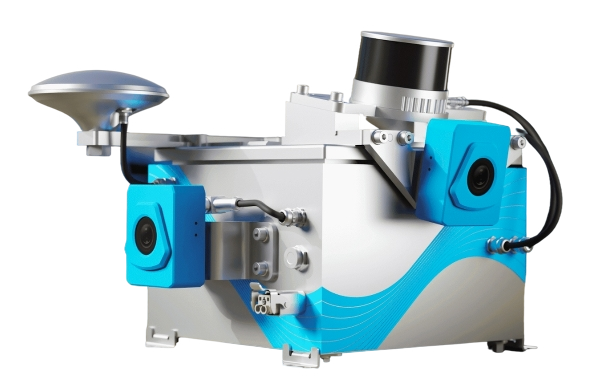
\includegraphics[width=0.6\linewidth]{images/sdx-compact-on-top-nobg.png}
    \caption[SDX-Compact]{The SDX-Compact manufactured by Sodex Innovations GmbH. The set of sensors consists of a 3D LiDAR scanner, three RGB cameras and a high-accuracy positioning system. Image source: \href{https://fieldwork.ch/de/produkte/geopositioning/mobile-datenerfassung/sdx-compact}{Fieldwork}}
    \label{fig:sdx-compact}
\end{figure}

\subsection{LiDAR Sensor}

The SDX-Compact \reffig{sdx-compact} is equipped with a Pandar XT32 \cite{hesai_xt16_32_32m} LiDAR sensor, manufactured by Hesai Technology. This is a mechanical rotating LiDAR with a full $360 \degree$ horizontal field of view and 32 beams distributed vertically, at $1 \degree$ resolution. With our settings, the sensor produces 10 complete scans per second, resulting in a horizontal resolution of $0.18 \degree$. The maximum operational range is 120m, decreasing to 50m for low-reflectivity targets. The official specifications state a typical accuracy of $\pm 1$cm, with precision $\pm 0.5$cm, in a static environment. For each beam, the strongest return is processed, leading to 640,000 points being generated per second. The high output bandwidth is handled by an Ethernet connection, over which points are sent as \acrshort{udp} packets. The sensor also supports \acrshort{ptp} synchronisation, essential for high-quality sensor fusion.


\subsection{GNSS/INS receiver}

Another component of the sensor stack is the Septentrio AsteRx SBi3 Pro+ GNSS/INS receiver \cite{Septentrio_AsteRx_SBi3_Pro+}, which provides global positioning and orientation data at a rate of 100Hz. Internally, this relies on two distinct mechanisms.

The localization information comes from a dual antenna GNSS module compatible with several GNSS consellations (e.g. \acrshort{gps}, \acrshort{glonass}, Galileo), to ensure optimal worldwide coverage. In standalone mode, the advertised typical accuracy is 1m, but the receiver also acts as an NTRIP (a protocol for differential GPS) client, gathering correction information, in order to achieve centimeter-level accuracy.

An \acrfull{imu} module records acceleration data and provides the remaining orientation angles (roll, pitch, yaw) to compute the complete pose, in 6 \acrfull{dof}. This is integrated with the absolute GNSS measurements using the patented FUSE+ technology \cite{Septentrio_FUSE_Sensor_Fusion}, resulting in an orientation error below  $\text{5-10}\degree$.

Like any system reliant on satellite communication, this will suffer significantly in situations where the signal propagation is disturbed (heavy clouds, ``urban canyons'', thick vegetation, spoofing), even leading to loss of \emph{\gls{gnssfix}}.

To conclude this section, we recognize and underline the importance of accurate extrinsic calibration between the LiDAR and the local INS coordinate frame, which has to be performed prior to any reliable data collection procedure. Given the radically different modalities of these two sensors, this is not a trivial task \cite{lidar-gps-calib} and lies outside the scope of the current work.

\begin{figure}[H]
    \centering
    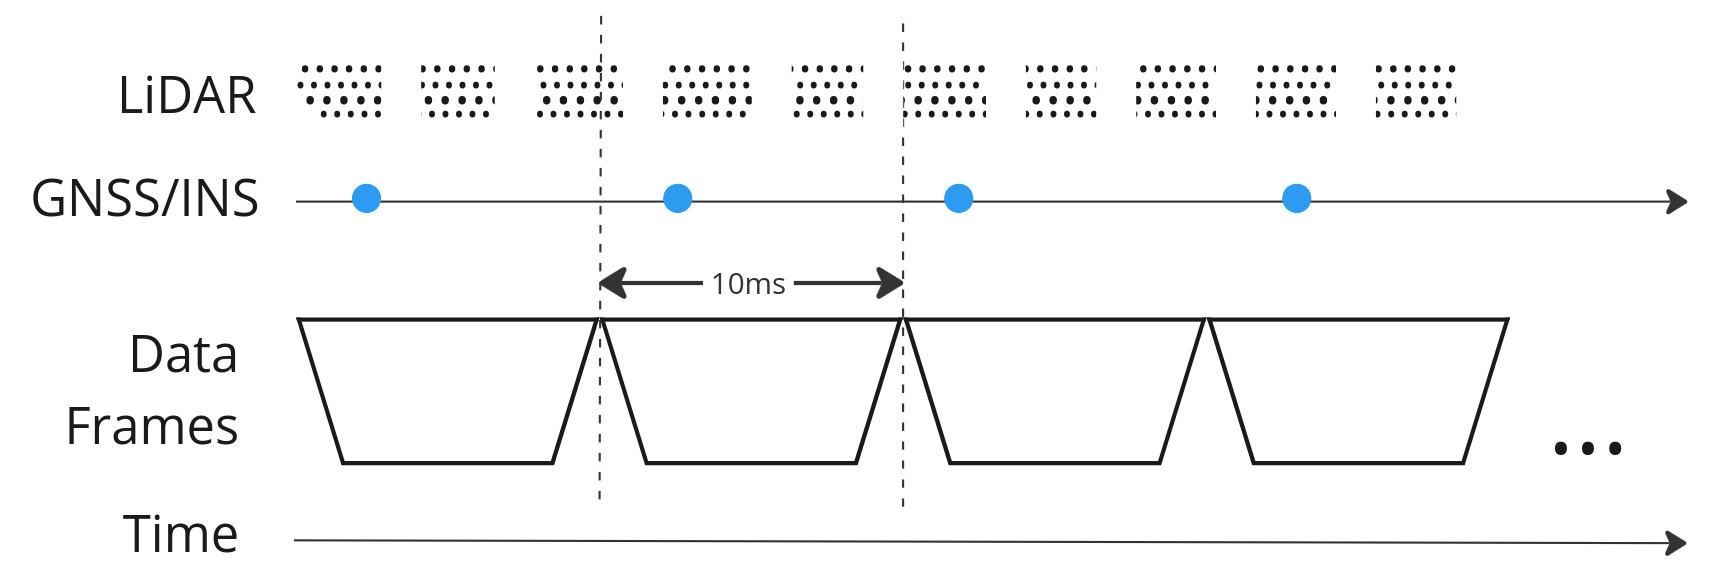
\includegraphics[width=0.7\linewidth]{images/data_sync.jpg}
    \caption[Data frame synchronisation]{A visualization of the data synchronisation process. Time is discretized into fixed-size intervals, resulting in data frames of custom resolution. These are populated with information from the two sensors: LiDAR points arrive as UDP packets, with one timestamp per packet, while GNSS readings have a frequency of approx. 100Hz. A data frame size of 10ms ensures that each interval has an associated GNSS measurement.}
    \label{fig:data-sync}
\end{figure}

\section{Data acquisition}

Data is collected by mounting the sensor rig on the roof of a vehicle, and driving around a target area. Through a high-speed mobile internet connection, the raw sensor output is uploaded to a cloud storage facility, and is later processed into a custom format that fuses the available information \reffig{data-sync}. This can occur because the sensors are PTP-synchronized on initialization, and all recorded data is timestamped.


\section{Solution architecture}






